

% !TeX root = RJwrapper.tex
\title{C443: An R-package to see a forest for the trees}
\author{by Aniek Sies, Kristof Meers and Iven Van Mechelen}



\maketitle

\abstract{
Classification trees, well-known for their ease of interpretation, are a widely used tool to solve statistical learning problems. However, researchers often end up with a forest rather than an individual classification tree, which implies a major cost due to the loss of the transparency of individual trees. Therefore, an important challenge is to enjoy the benefits of forests without paying this cost. In this paper, we propose the R-package \pkg{C443}. The C443 methodology simplifies a forest into one or a few condensed summary trees, to gain insight into its central tendency and heterogeneity. This is done by clustering the trees in the forest based on similarities between them, and on post-processing the clustering output. We will elaborate upon the implementation of the methodology in the package, and will illustrate its use with three examples.
}

\section{Introduction}
Classification trees are a widely used tool in the statistical learning of the relationship between a set of predictor variables and a categorical outcome \citep{Breiman1984, Quinlan1986}. A particularly attractive feature is that they typically lead to insightful and well interpretable results.

However, researchers often end up with a forest (i.e., a set of multiple trees) rather than with a single classification or decision tree. There are several reasons for this: First, single trees are known to be fairly unstable (e.g., \citet{philipp2016, philipp2018}); we may wish to investigate this instability through the creation of a forest by bringing about small changes in the learning sample (e.g., drawing bootstrap subsamples) or in the tree building process (e.g., varying tuning parameters)\citep{Breiman1996a, Strobl2009, Turney1995}. Second, we may wish to improve prediction accuracy \citep{Bauer1999, Dietterich2000, Hastie2009, skurichina2002} by generating a forest by means of ensemble methods such as random forests \citep{Breiman2001}, bagging \citep{Breiman1996b}, or boosting \citep{Freund1997}. Third, if there are multiple outcomes, we may wish to grow one or multiple trees for each outcome variable, leading once again to the formation of a forest. Fourth, in order to deal with missing data, one preferred method is multiple imputation \citep{Rubin1987}, resulting in several imputed data sets, based on each of which we can construct a classification tree.

All four of these are excellent reasons to prefer forests over single trees. Nonetheless, forests have a major cost that is implied by a complete loss of the transparency of single trees. This brings about the challenge to look for ways to enjoy the benefits of a forest without having to pay this cost.

More specifically, one may wish to capture three sorts of insight from a forest:
\begin{enumerate}
\item{Central tendency: Can a forest be summarized in one or a few central decision structures and how do these look like?}
\item{Heterogeneity: How much variability is there in the forest and what are its contents? For example, are all trees in the forest slight variations on one central decision structure, or are they subject to sizeable qualitative differences?}
\item{Linking heterogeneity to tree covariates: In case of a heterogeneous forest based on known sources of variation (e.g., different types of tuning parameters or response variables), are qualitative within-forest differences related to this variation source? For example, do different response variables result in different decision structures?}
\end{enumerate}

Partial answers to this challenge can be found in earlier work. As such, variable importance measures have been proposed to capture the most central predictor variables in random forests \citep{Breiman2001, Breiman2003}. From their part, \citet{Banerjee2012, Briand2009}, and \citet{Chipman1998} suggested to select one or a few summary trees within a forest based on ad hoc calculated similarities between the individual trees, whereas \citet{philipp2016} developed a methodology and associated R-package \pkg{stablelearner} to visualize and summarize variable and split point within-forest heterogeneity. This is useful in evaluating stability of tree splits in terms of split variables and/or split-points, but does not evaluate stability of entire tree structures. A lasso regression methodology \citep{Friedman2008} along with the associated R-package \pkg{pre} \citep{Fokkema2020}, has been proposed to derive a sparse ensemble from an initially large prediction rule ensemble. Although this results in an easily interpretable rule, it does not give insight into the heterogeneity within the initial rule ensemble. Quite a different approach is taken in the area of interpretable machine learning, where local SHapley Additive exPlanations (SHAP) of ensemble learners are looked for in the form of additive contributions of input features to estimated risk scores (e.g., \citet{Lundberg2020}).

A comprehensive and complementary way to recover insight from a forest could be obtained by means of a methodology proposed by \citet{Sies2020}. Unlike the SHAP-approach, the C443 methodology focuses on global rather than local explanations, remains within a tree context instead of moving to an additive framework, and targets categorical outcome variables rather than unidimensional risk scores. The methodology comprises three components:
\begin{enumerate}
\item{Similarities calculation between all trees in the forest. A complication at this point is the vast range of similarity measures that can be invoked within a tree context, as the choice of a similarity measure has major consequences for the output of the methodology and its interpretation. \citet{Sies2020} developed a novel, comprehensive conceptual framework to cope with this complication and assist the user in making a thoughtful choice of a suitable similarity measure.}
\item{A similarity-based clustering of the trees in the forest, where, given the critical concern about insightfulness, clusters that are well interpretable regarding the underlying decision structure and the relation between the predictors and the categorical response variable are obtained.}
\item{A post-processing of the clustering result to arrive at the essential insights into central tendency and heterogeneity looked for.}
\end{enumerate}

The aim of the current paper is to introduce the R-package \pkg{C443}, which implements the methodology proposed by \citet{Sies2020}. The package is available from the Comprehensive R Archive Network (CRAN) on \url{https://CRAN.R-project.org/package=C443} and is also accessible through Github (\url{https://github.com/KULeuven-PPW-OKPIV/C443}).The package accepts as input user-supplied forests with a wide range of formats (in part making use of the \pkg{partykit} package \citep{Hothornb2015}), and a user-provided similarity matrix between the forests' trees based on a similarity measure of the user's choice (if available), and covariate information on the trees (if available). Otherwise, it  also includes the option to calculate a matrix of similarities between the trees of the user-supplied forest based on one out of eight possible similarity measures within the conceptual framework proposed by \citet{Sies2020}. The package further partitions the trees in the forest under study into a few well-interpretable clusters (based on the user-provided or calculated similarities), using the PAM algorithm \citep{Kaufman2009} implemented in the \pkg{cluster} package \citep{Maechler2019}. Finally, it includes a number of methods and functions that can be used for post-processing the clustering output to summarize the forest, capture within-forest heterogeneity, or link this heterogeneity to tree covariates.


\section{C443 Methodology} \label{sec:methodology}
In this section we will briefly recapitulate the main concepts of the methodology proposed by \citet{Sies2020}.

\subsection{Similarities}
Any set of categories or concepts has two sides: the side of the categories' meaning in terms of their defining or characteristic features, and the side of the categories' membership (with the two sides in question being referred to as the categories' intension and extension, respectively: \citet{leibniz1764}). In line with this, when evaluating similarities between classification trees, we could do so with respect to the trees' meaning (i.e., their predictor-related contents), with respect to the classifications of the objects or experimental units implied by them, or with respect to a hybrid combination of both facets.

When considering to evaluate tree similarities with respect to common predictor-related contents, two groups of questions are further to be addressed:
\begin{enumerate}
\item{Does one want to calculate similarity in terms of shared predictor variables only or also in terms of shared split points on common predictors? Furthermore, in the latter case, is one willing to take into account a tolerance zone when evaluating equality of split points?}
\item{Does one want to calculate similarity in terms of individual predictors or rather in terms of sets of predictors as implied by the definitions of each of the leaves of the trees under study? In the latter case, is one willing to take into account: (a) the order of the predictors on the downward path from the root to the leaf under study, and (b) the relevant part of the predictor range (i.e., lower vs. upper part) involved in the definition of the leaf in question?}
\end{enumerate}
These two groups of questions are schematically represented in Figure \ref{figSim1}. Orthogonally combining all 3*5 possible answers to them yields 15 possible similarity types.

\begin{figure}[H]
	\centering
	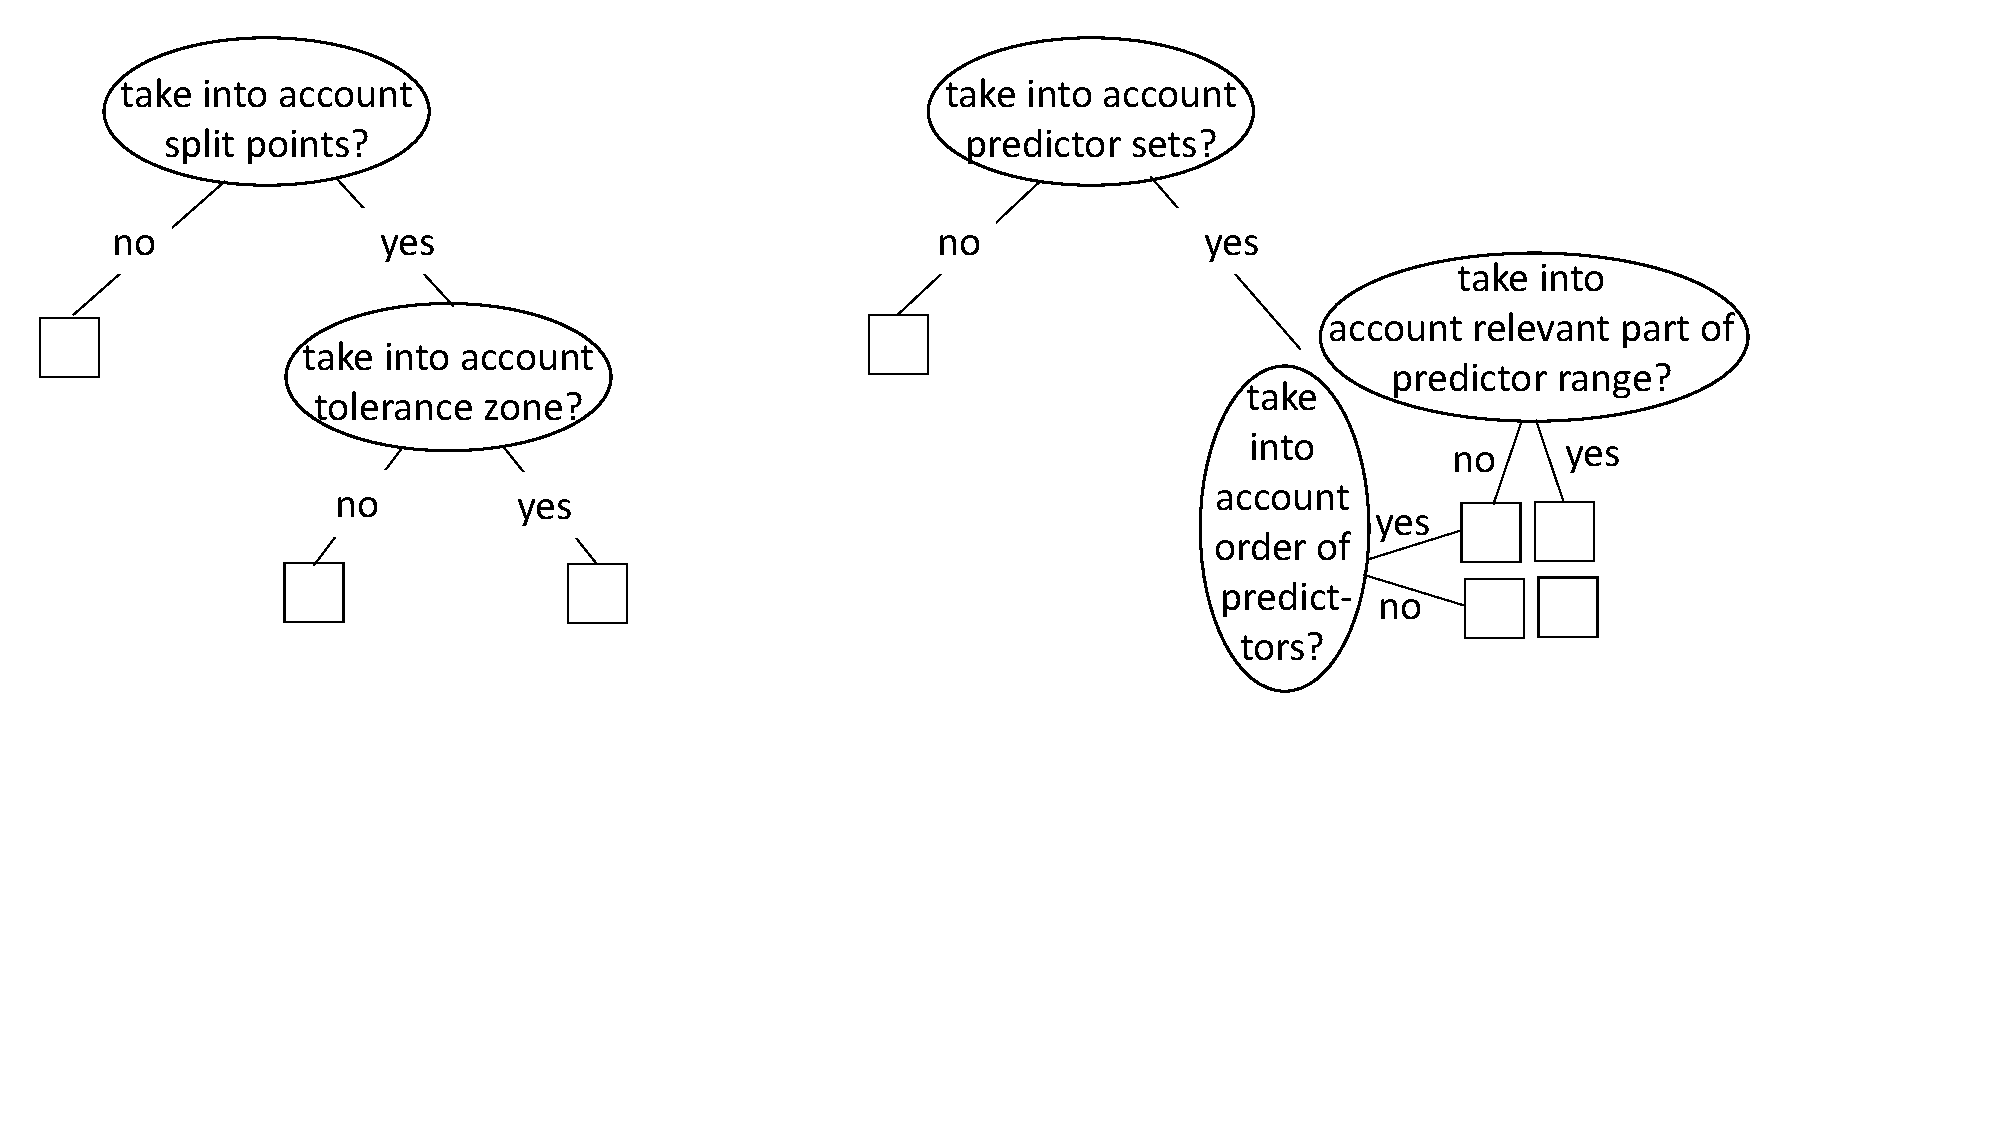
\includegraphics[width=\linewidth, trim=0 7cm 0 0, clip]{sim2.pdf}
	\caption{Schematic representation of two groups of questions within comprehensive conceptual framework with regard to tree similarities in terms of shared predictor-related contents.}
	\label{figSim1}
\end{figure}

When evaluating the similarity between two trees with respect to the classifications of the objects or experimental units implied by them, in general, pairs of objects that belong to the same class in each of the two trees will contribute to a higher similarity. Two questions should further be addressed for similarities with regard to implied class memberships:
\begin{enumerate}
\item{Does one want to consider the classifications (partitions) of the experimental units by the class labels or the leaf memberships?}
\item{Should one factor in pairs of objects that belong to the same class in each of the two trees under study only if these classes are associated with the same class label across the two trees?}
\end{enumerate}
These two questions are schematically represented in Figure \ref{figSim2}. Orthogonally combining all 2*2 possible answers to them yields 4 possible similarity types.


\begin{figure}[H]
		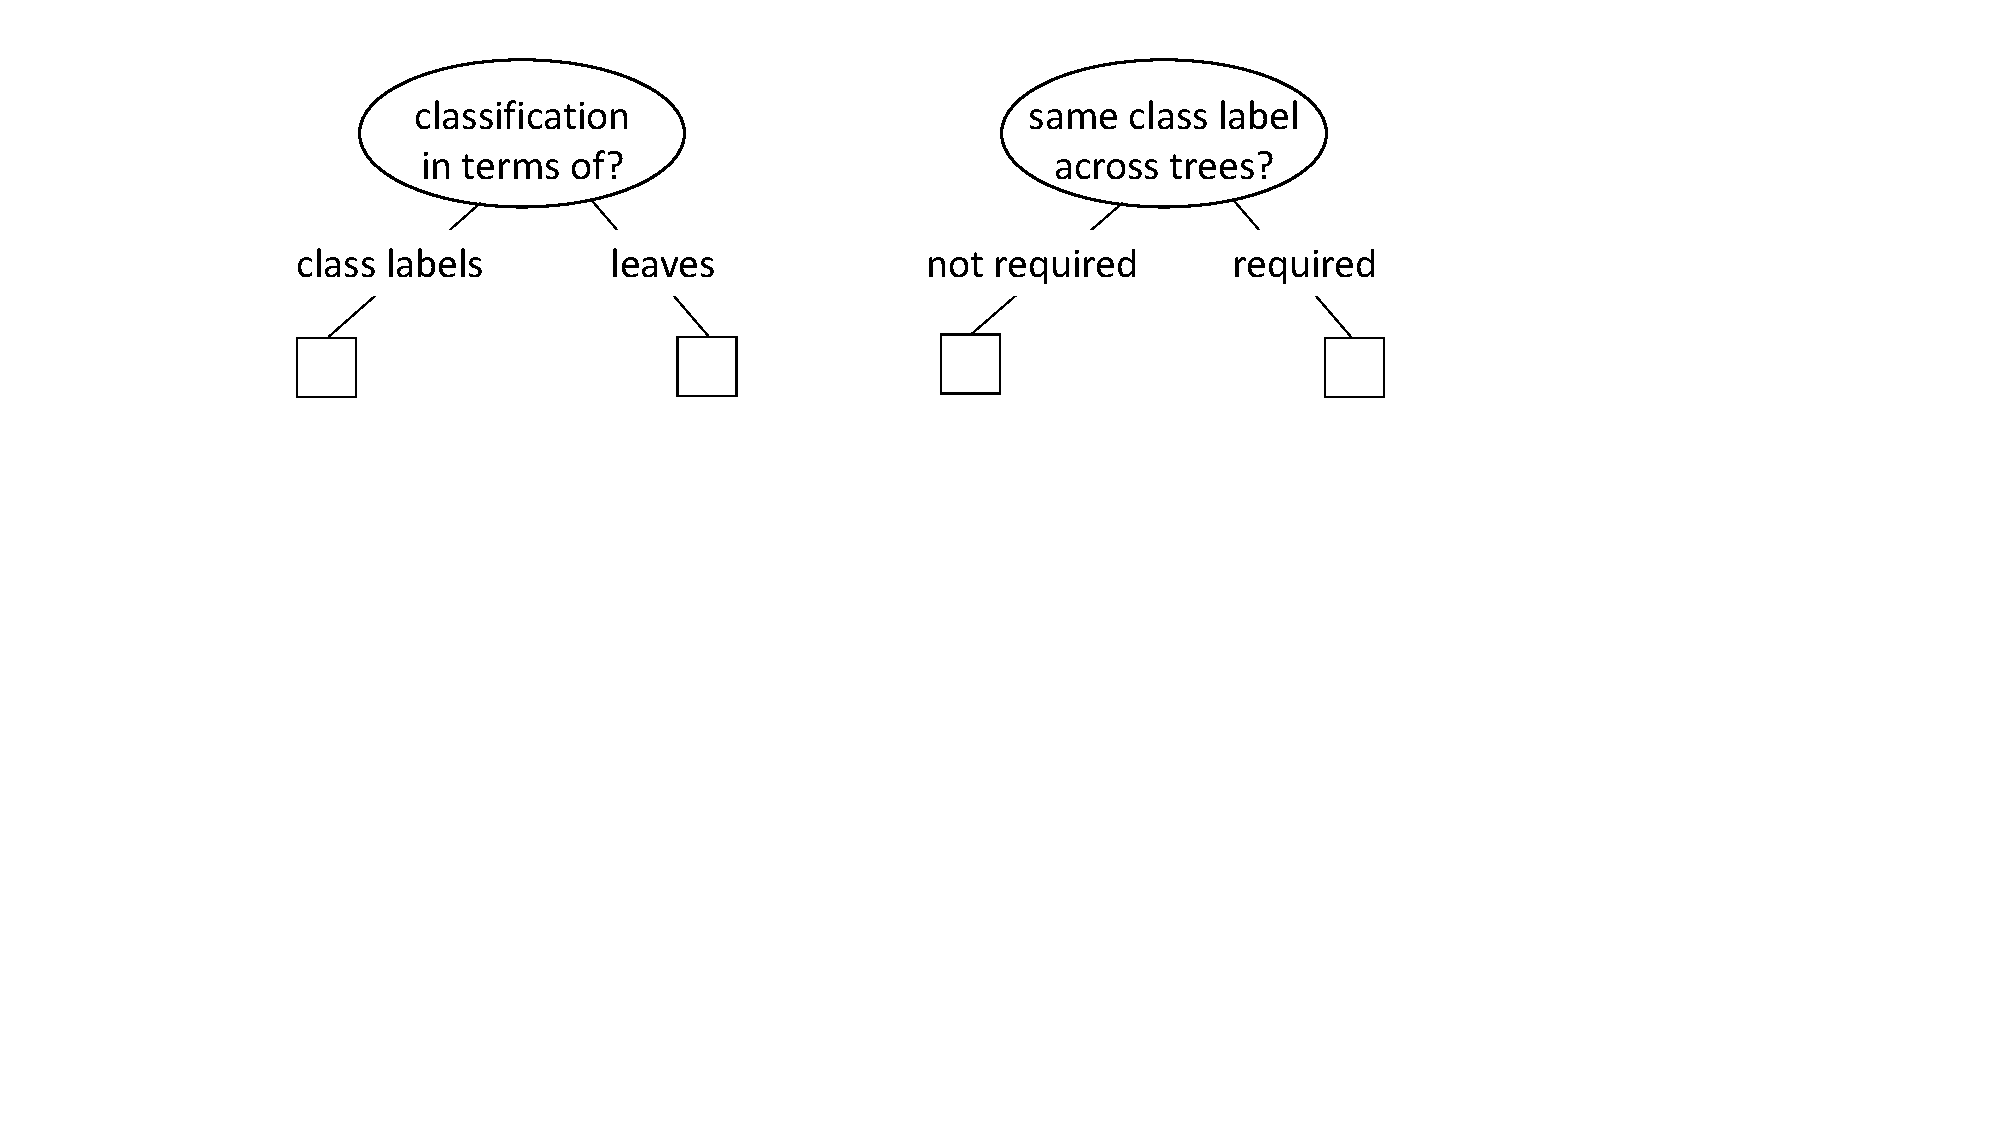
\includegraphics[width=\linewidth, trim=0 11cm 0 0, clip]{similarities.pdf}
	\caption{Schematic representation of two questions within comprehensive conceptual framework with regard to tree similarities in terms of agreement between implied classifications.}
	\label{figSim2}
\end{figure}


To illustrate the above, let us briefly consider three examples. As a first example, \citet{Shannon1999} proposed to define a dissimilarity $d(T_1, T_2)$  between two trees $T_1$ and  $T_2$ as:
\begin{equation}
d(T_1, T_2) = \sum_{r}{\alpha_r |D^r_{T_1,T_2}|},
\end{equation}
where $|D^r_{T_1,T_2}|$ equals the number of distinctive paths of length $r$ from a root node to a leaf, with a path denoting an ordered set of relevant predictor parts (upper vs. lower) as implied by a leaf, with distinctive meaning that the path shows up in one of the two trees only, and with $\alpha_r$ denoting a set of prespecified weights (e.g., $\alpha_r = \frac{1}{r}$). Obviously, this is a dissimilarity measure that captures the trees' meaning or predictor-related contents only, that does not take into account split points, that does take into account predictor sets, and while doing so does take into account both the order and the range-part (lower vs. upper) of the predictors.

As a second example, while denoting the set of objects under study by $\{o_1,...,o_i,...,o_n\}$, \citet{Chipman1998} defined a dissimilarity $d(T_1, T_2)$ between two trees $T_1$ and $T_2$ as:
\begin{equation}
d(T_1, T_2)= \frac{\sum_{i>i'}|I^{T_1}(o_i, o_{i'}) - I^{T_2}(o_i, o_{i'}) |}{\binom{n}{2}},
\end{equation}
with $I^{T_j}(o_i, o_{i'}) = 1$ if $o_i$ and $o_{i'}$ belong to the same leaf in $T_j, j=1,2$, and  $I^{T_j}(o_i, o_{i'}) = 0$ otherwise. Obviously, this is a dissimilarity measure that captures the trees' implied classifications only, while considering classifications implied by leaf membership without requiring equality across trees of class labels associated with the leaves. Note that, if different observations were used to create the trees under study (e.g., in case of a forest based on bootstrap samples), the observations $o_i$, $i=1,...,n$ are those from the original data set (e.g., the data set from which the bootstrap samples were drawn).

As a third example, we consider a hybrid tree similarity measure $sim_T(T_1,T_2)$ implemented in the package \pkg{C443}. This measure is based on a leaf similarity measure $sim_L(l,l')$ that captures predictor-related contents in terms of the (frequencies of occurrence of the) combinations of predictors and range-parts (lower vs. upper) $PRP_p$ associated with leafs $l \in T_1$ and $l' \in T_2$ (while leaving aside split points and the order of the predictors), and that captures the trees' implied classifications by assuming a leaf similarity value of zero for leafs that are associated with different class labels (i.e., $c(l) \neq c(l')$). Specifically, if $T_1$ and $T_2$ both have height zero (i.e., consist of a root node only), by definition $sim_T(T_1,T_2)=1$. Otherwise, $sim_T(T_1,T_2)$ is based on leaf similarity measure $sim_L(l,l')$, with:
\begin{equation}
sim_L(l,l')=\begin{cases}
\frac{\sum_{p} min (\#^{l} PRP_p, \#^{l'} PRP_p)}{\sum_{p} max (\#^{l} PRP_p, \#^{l'}PRP_p)} & \text{if } c(l) = c(l') \\ \\
0 & \text{otherwise},
\end{cases}
\end{equation}
with $\#^{l}PRP_p$ (resp. $\#^{l'}PRP_p$) denoting the frequency of occurrence of the $p^{th}$ predictor range-part combination $PRP_p$ in the definition of leaf $l$ (resp. $l'$). The tree similarity $sim_T(T_1,T_2)$ then relies on the search for an optimal matching between (subsets of) the leafs of $T_1$ and $T_2$, $S_{L_{T_1}} \subset L_{T_1}$ and $S_{L_{T_2}} \subset L_{T_2}$, as formalized by a bijection $g: S_{L_{T_1}} \to S_{L_{T_2}}$. Specifically:
\begin{equation}
sim_T(T_1,T_2)={\underset{g:~S_{L_{T_1}} \overset{\text{bijection}}\longrightarrow S_{L_{T_2}} }\max\frac{\sum_{l \in S_{L_{T_1}}sim_L(l,g(l))}}{min(\#L_{T_1},\#L_{T_2})}}.
\end{equation}


\subsection{Clustering}
A second step in the proposed methodology consists of a clustering (viz., a partitioning) of the forest based on the similarity measure chosen in the first step. A major challenge at this point is the interpretability of the resulting clusters. For this purpose, Partitioning Around Medoids (PAM, \citet{Kaufman2009}) was chosen as a clustering method. In this method, each cluster is centered around a medoid, which is an actual element of the cluster (unlike the centroids in other clustering methods). Given a (dis)similarity matrix and a prespecified number of clusters $k$, PAM looks for $k$ medoids that are such that a loss function consisting of the sum across all objects of the dissimilarity between the object and its closest medoid is minimized. PAM starts with an initial selection of $k$ medoids, and subsequently replaces iteratively each medoid by the object that minimizes the loss function until no further improvement in the loss function is observed.

The key advantage of using PAM to cluster a forest, is that PAM leads to a set of clusters each of which is represented by a cluster member, that is to say, a well-interpretable tree (which means that an insightfulness baby is rescued out of the bathwater of the forest!). To be sure, when interpreting the medoid trees resulting from PAM, one should never forget the (dis)similarity type on which the clustering was based. For example, if a similarity was used that exclusively reflected the objects' classifications, then an interpretation of the predictor-related contents of the medoid trees is simply not admissible. Indeed, the trees within each cluster will then be similar in terms of implied classifications, but may be very different with respect to predictors and split points.



\subsection{Post-processing}
To retrieve critical insights into the central tendency and heterogeneity of the forest under study, a suitable post-processing of the clustering output is called for. Below, we will list a few useful questions and steps at this point. For all of them, we must again emphasize the importance of keeping aware of the chosen similarity at the basis of the clustering, as this may strongly constrain which kinds of interpretation of the post-processed output will be admissible. (To overcome these constraints, one either has to do all of the similarity and clustering calculations over with a different type of tree similarity measure, or to revert to hybrid types of similarity measures that tap both predictor- and classification-related aspects of the trees under study.)

The most obvious place to grasp the central tendency of the forest in focus is the medoid of the one-cluster solution. Besides, one could also take a look at the medoids of solutions with a few more clusters and inspect which aspects all medoids in question have in common. 

Concerning within-forest heterogeneity, to start with, one can examine this quantitatively in terms of the amount of variability at play. A straightforward question at this point is how many clusters are needed to summarize the forest. Determining the optimal number of clusters is a common challenge in the clustering domain, for which a very broad range of measures and heuristic procedures (or "stopping rules") have been proposed. Within the methodology proposed by \citet{Sies2020}, three types of plots corresponding to different values of the number of clusters, $k$, may be singled out:
\begin{enumerate}
	\item a plot of the average within-cluster similarities (or, alternatively, the average similarities between the cluster elements and their cluster medoids) for the similarity measure at the basis of the clustering; in general, we recommend to select the number of clusters based on one of these plots because of their direct link with the loss function that is optimized by the PAM algorithm
	\item a plot of the Average Silhouette Width (ASW, \citep{Rousseeuw1987}), that is, the average of all objects' silhouette; the silhouette of an object is a function of its mean similarity to the objects of its own cluster minus its mean similarity to the objects of its second closest cluster; ASW is recommended by the authors of PAM and the corresponding R-package \citep{Kaufman2009, Maechler2019}
	\item  suppose that the forest under study was created to arrive at a better prediction accuracy and that a similarity measure was chosen or constructed that (also) captures agreement between classifications in terms of class labels; in this scenario, we recommend determining the number of clusters also by examining: (a) a plot depicting the accuracy of the predicted class labels (for the originally observed dataset), based on combining the predictions of the first $k$ medoid trees (weighted by their corresponding cluster cardinalities), and (b) a plot of the agreement between the class label for each object of the originally observed dataset, predicted on the basis of the random forest as a whole versus the class label predicted on the basis of the first $k$ medoid trees (weighted by their corresponding cluster cardinalities). \end{enumerate}
Another potential quantitative approach to assess forest heterogeneity involves examining the cluster sizes in solutions where k>1. For example, solutions with a single very dominant cluster (in terms of cluster size), would point at considerable within-forest homogeneity.

We can further also try to capture within-forest heterogeneity from a qualitative perspective, that is, the contents of the within-forest differences. In view of this, one may compare the cluster medoids, once more aligning with the selected similarity measure, in terms of their predictor-related contents, and/or predicted class labels. With regard to predictor-related contents, possible outcomes could be that all medoids constitute only minor variations on a common topology (e.g., in terms of a small number of distinctive secondary splits in different medoids), versus major variations that involve very different kinds of predictors and split points. With regard to predicted class labels, the predictions of the medoids can be compared in terms of  marginal totals of all class labels per medoid as well as in terms of a contingency table with the numbers of experimental units assigned to each combination of class labels by each of two or more different medoid trees. A possible outcome could be that the classifications implied by one medoid are only a refinement of these implied by another medoid, with the majority of observations being assigned by both to the same class label.

Finally, one may wish to investigate the link between covariate information on the trees in the forest and within-forest heterogeneity, in case such covariate information is available. First of all, one may wish to do so in terms of the relation between covariates and cluster membership. In case of a discrete covariate (e.g., the nature of the outcome variable), this may lead to questions such as "Do trees based on a same value of the covariate mainly end up in the same cluster?", or, more in general, "Which values of the covariate lead to trees in the same cluster and which values to trees in different clusters?". In case of a continuous covariate (e.g., the value of some tuning parameter in the tree building algorithm): "Does cluster membership relate to this covariate (e.g., by comparing within- and between-cluster differences with regard to it)?". Second, if a relationship between cluster membership and a covariate would be established, then the relationship between that covariate and the predictor-related contents or implied classifications of the cluster medoids could be examined (in accordance with the chosen similarity measure). As an example, if the covariate would pertain to different outcome variables, one might wish to examine differences between these outcome variables in terms of their predictive basis (if the chosen similarity measure would allow the researcher to do so).


\section{Implementation of the methodology in C443} \label{sec:implementation}
In this Section, we will discuss how the methodology described above has been implemented in the R-package \pkg{C443}. First, we will describe user input when employing the package. In the following subsections, we will discuss how the different constituents of the methodology (i.e., the calculation of similarities, the clustering, and the post-processing of the clustering output) have been implemented in the package.


\subsection{Input needed for the package}
Users of the package \pkg{C443} should provide at least one mandatory piece of input, namely the forest of interest. In addition, two optional pieces of input may be supplied: a similarity matrix and covariate information on each tree in the forest.

\subsubsection{Forest}
There are many techniques and associated R-packages to grow classification trees. For example, Classification and Regression Trees \citep{Breiman1984} can be grown using \pkg{rpart} \citep{therneau2019}, Conditional inference trees \citep{Hothorna2006} using \pkg{partykit} \citep{Hothornb2015}, and C4.5 trees \citep{Quinlan1993} using \pkg{RWeka} \citep{Hornik2009}. 


Likewise, many techniques and R-packages exist to create a forest. First, creating a forest to investigate instability of trees can be done in several ways. One could grow trees using one of the packages mentioned above on sub-samples obtained from the \texttt{sample} function with \texttt{replace = FALSE} and \texttt{size} < \textit{n} (where \textit{n} is the size of the original data set), or on bootstrap samples obtained from the same function with \texttt{replace = TRUE} and \texttt{size} = \textit{n}. Second, to create a forest in view of improving prediction accuracy, one may employ boosting \citep{Freund1997}, as implemented in R-packages such as \pkg{adabag} \citep{Alfaro2013} and \pkg{gbm} \citep{ridgeway2007}. or random forests \citep{Breiman2001}, as implemented in the packages \pkg{randomForest} \citep{Liaw2002}  and \pkg{ranger} \citep{Wright2017}. Third, a forest can result from growing trees on a number of different outcome variables. Fourth, multiple imputation \citep{Rubin1987} can be applied in case of missing data using the \pkg{mice} package \citep{VanBuuren2011}, and subsequently a tree can be grown on each imputed data set, which would return a forest as well.

The \pkg{C443} package does not have a specific functionality for creating forests, given the large variety of techniques and available R-packages to do so. Rather, a multitude of types of forests are accepted as input by the package, where three pieces of information are required:
\begin{enumerate}
    \item the entire set of observed data at the basis of the forest, stored as a data frame --in case of a forest produced by bringing about small changes in the learning data (e.g., by taking bootstrap samples from the set of experimental units), this would be the entire originally observed data set; in case of a forest based on multiple outcomes, this would be the data set with inclusion of all outcomes; and in case of a forest as a result of multiple imputation, this would be the originally observed data set without imputations--; 
    \item the \textit{n} trees in the forest, stored as a list of party objects, or of objects inheriting from party objects (included but not limited to \pkg{glmtree}, \pkg{ctree}), or of objects that are convertible into party objects using 
    \begin{enumerate}
        \item \pkg{partykit} \citep{Hothornb2015}): for rpart and J48 objects
        \item \pkg{C443}'s internal functions: for randomForest and ranger objects, including ranger objects that can be delivered from  packages such as DFNET \citep{Pfeifer2022};
    \end{enumerate}
    (the class of the first tree is checked in \pkg{C443} with the \texttt{class} function); 
    \item if not included in the party object (e.g., when \pkg{rpart} was used to grow the trees), the \textit{n} data sets on which the individual trees in the forest were based, stored as a list of data frames. 
\end{enumerate}


\subsubsection{Similarity matrix}
Users can provide a home-made similarity matrix as input for the clustering. This square matrix with number of rows/columns  equal to the number of trees in the forest,  must be symmetric. The similarity values should vary between 0 and 1 (with 0 indicating no similarity at all and 1 indicating a perfect similarity). Otherwise, quite a few tree dissimilarity measures have been proposed, which often vary between 0 and 1 (with 0 indicating no dissimilarity at all and 1 full dissimilarity). We can transform these into similarities by subtracting them from 1.

\subsubsection{Covariate information}
If the user is interested in relating the possible heterogeneity within the forest to values of the trees on one or more covariates, a vector or dataframe with the values of those covariates for each tree should be provided.

\subsection{Similarity calculation}
There is the option to have \pkg{C443} calculate a similarity matrix alongside the option of a user-provided similarity matrix. For this purpose, eight similarity measures proposed by \citet{Sies2020} have been implemented in the package, each of which takes into account different aspects of similarity. In Table \ref{tab:00}, we describe each implemented similarity measure. (In the Supplementary Materials, mathematical formalizations are given.)


\begin{table}[t!]
	
	\centering
		\caption{\label{tab:00} Overview of similarity measures implemented in \pkg{C443}.}
	\begin{threeparttable}
	\begin{tabular}{llp{10cm}}
		\hline
		No\tnote{1} & Similarity Respect           & Basis  \\ \hline
		1 &Predictor content &		$\#$ common predictors  \\
		2 & Predictor content &		$\#$ common predictor-split point combinations \\
		3 &	Predictor content &	$\#$ distinctive ordered sets of predictor-range part combinations \\
		4 &	Classifications &	agreement of partitions implied by leaf membership \\
		5 &	Classifications &	agreement of partitions implied by class labels \\
		6 &	Hybrid &	$\#$ predictor-range part occurrences in definitions of leaves with same class label \\
		7&	Hybrid & $\#$ predictor-split point combinations in definitions of leaves with same class label \\
		8 &	Hybrid & closeness to logical equivalence (applicable in case of binary predictors only)\\
		\hline
	\end{tabular}
\begin{tablenotes}\footnotesize
	\item[1] Number of section in Supplementary Materials that includes mathematical formalization and reference citation for measure in question
\end{tablenotes}

\end{threeparttable}
\end{table}


\subsection{Clustering}
Starting from a dissimilarity matrix (viz., 1 - the similarity matrix provided by the user or calculated by the package), a clustering of the trees in the forest is done based on the PAM algorithm \citep{Kaufman2009}, as implemented in the \pkg{pam} function of the \pkg{cluster} package \citep{Maechler2019}. The original PAM algorithm consists of two phases: a BUILD phase (an intelligent way of finding an initial set of clusters), and a SWAP phase (swapping medoids and candidate medoids until convergence). 

To lower the risk of ending up in a local minimum, we implemented a multi-start approach. In addition to the BUILD phase, we use 1000 starts where the initial cluster medoids are randomly assigned. Next, for each of the 1001 initial sets of medoids, we use SWAP until convergence. Finally, the solution that yields the lowest value of the objective function across all starts is retained.

For PAM with a BUILD start, we use \texttt{medoids=NULL} and set \texttt{do.swap=TRUE}. To run PAM with random starts, we assign random initial values for the medoids using \texttt{medoids= randomstarts}. Here, \texttt{randomstarts} is a vector with \textit{k} values, randomly sampled without replacement from 1 to T, where $k$ is the number of medoids and \textit{T} is the number of trees in the forest. For reproducibility purposes, the seed number is included in the final solution. Finally, we always use \texttt{pamonce=3} to speed up the SWAP phase, as suggested by \citet{schubert2019}.

The procedure described above is repeated for each number of clusters between the minimum and maximum
number of clusters specified by the user. For each number of clusters, the clustering result is returned as a \texttt{clusterforest} object. 



\subsection{Post-processing}
The two main insights looked for (central tendency and forest heterogenoneity) can be captured by post-processing the clustering result using several functions on the \texttt{clusterforest} object.

\subsubsection{Central tendency}

The function \texttt{medoidtrees()} returns the medoid tree(s) of a given \texttt{clusterforest} solution as party object(s). The function \texttt{plot()} may be used to plot the medoids, and the \texttt{predict()} function to obtain their implied classifications.


\subsubsection{Heterogeneity}
Regarding quantitative heterogeneity, first, in order to decide on the number of clusters needed to summarize the forest, one can use the function \texttt{plot()} with the \texttt{clusterforest} object as the only argument. This will return two plots that visualize for each solution: 1) the average within-cluster similarity, and 2) the ASW \citep{Rousseeuw1987}; optionally, a third and fourth plot can also be returned, which show for each solution the accuracy of the predicted class labels (for the originally observed dataset) based on the medoid trees, and the agreement in classifications based on the medoids only versus based on the full forest (see Section 2.3). Second, the cluster sizes can be obtained by extracting the cluster assignment of all trees for a given solution from the \texttt{clusterforest} object using the \texttt{clusters()} function, and subsequently counting the number of trees assigned to each cluster.

Regarding qualitative heterogeneity, the medoids' predictive content and classifications can again be obtained by means of the functions \texttt{medoidtrees()}, \texttt{plot()} and \texttt{predict()}. 
Finally, to explore the relationship between one or more tree covariates and the heterogeneity within the forest, the function \texttt{treesource()} can be employed. In case of a discrete covariate, it visualizes the number of trees that belongs to each cluster for each value of the covariate. In case of a continuous covariate, it returns the mean and standard deviation of the covariate within each cluster. One can further interpret the relation between the covariate and the clusters by utilizing the cluster medoids' predictive contents and/or implied classifications. This can be done using a combination of the functions \texttt{medoidtrees()}, \texttt{plot()} and \texttt{predict()}.


\section{Practical usage of the R-package} \label{sec:illustrations}
We will illustrate the use of the R-package with three real data examples taken from the Drug Consumption data set \citep{Fehrman2017}. This data set is freely available from the UCI Machine Learning Repository \citep{Dheeru2017} and is included in a slightly transformed format in \pkg{C443}. The data set contains anonymous survey data from 1885 respondents, who reported on their use of different types of drugs. Although in the original data set each of the drug-use variables had seven response categories (never used, used over a decade ago, used in the last decade, year, month, week or day), we included them as binary response variables in the R-package, with categories non-user (never used or used over a decade ago only) versus user (all other categories), similar to \citet{Fehrman2017}.

In the first and second example, we will focus on one drug only, namely ecstasy. In the third example, we will broaden the scope of the application to the use of several drugs, viz., amphetamines, benzodiazepines, ecstasy, LSD and mushrooms.
Finally, in all three examples we will use as predictors a number of demographic variables (age, gender, level of education), the Big Five personality traits (i.e., Extraversion, Agreeableness, Conscientiousness, Neuroticism, and Openness to experience) measured by the NEO-FFI-R \citep{McCrae2004}, Impulsivity measured by the BIS-11 \citep{Patton1995}, and Sensation seeking measured by the ImpSS \citep{Zuckerman1993}. Note that all predictors were initially categorical (ordinal or nominal) and were quantified by \citet{Fehrman2017}.

\subsection{Example 1: Assessing stability} \label{sec:illustration1}
The goal of  the first  analysis is to find out which types of persons are at risk of using ecstasy. Although this question can be insightfully addressed by growing a single classification tree on the full data set, the interpretation of the result may be undermined by the issue of tree instability. We will therefore investigate the stability of the obtained solution using \pkg{C443}. 
Specifically, we will draw 100 bootstrap samples and grow a classification tree on each sample. Next, we will use \pkg{C443} to calculate similarities between the resulting trees, and subsequently cluster them. Finally, we will post-process the obtained cluster result to gain insight into the central tendency and heterogeneity of the forest. 

We first load the package \pkg{C443}, and extract the relevant information for this analysis from the drugs data set: 

\begin{example}

R> library (C443)
R> EcstData = drugs [, c("Age", "Gender", "Edu", "Neuro", "Extr", "Open", "Agree",
+    "Consc", "Impul", "Sensat", "Ecst")] 
R> EcstData$Ecst <- as.factor(EcstData$Ecst) 
R> head(EcstData, 3)


       Age   Gender      Edu    Neuro     Extr     Open    Agree
1  0.49788  0.48246 -0.05921  0.31287 -0.57545 -0.58331 -0.91699
2 -0.07854 -0.48246  1.98437 -0.67825  1.93886  1.43533  0.76096
3  0.49788 -0.48246 -0.05921 -0.46725  0.80523 -0.84732 -1.62090
     Consc    Impul   Sensat Ecst
1 -0.00665 -0.21712 -1.18084    0
2 -0.14277 -0.71126 -0.21575    1
3 -1.01450 -1.37983  0.40148    0

\end{example}
To answer the question of which types of people may be at risk for ecstasy use, we first grow a single decision tree on the full data set using \pkg{rpart}. We prune the resulting tree using the complexity parameter associated with a cross-validated prediction error that is maximally one standard error higher than the lowest one (as suggested by \citet{Hastie2009}). We plot the result using \pkg{partykit}:
\begin{example}
R> library(rpart)
R> library(partykit)
R> set.seed(123)
R> EcstTree <- rpart(Ecst ~ ., data = EcstData, control = rpart.control(
+    minsplit = 100, maxdepth = 3, maxsurrogate=0, maxcompete=0))
R> cp <-EcstTree$cptable[order(EcstTree$cptable[1:which.min(EcstTree$cptable[, "xerror"]), "xerror"]), ]
R> maxcp <- cp[1, "xerror"] + 1.96 * cp[1, "xstd"]
R> cp <- cp[as.numeric(which.max(1 / (maxcp - cp[, "xerror"]))), "CP"]
R> PrunedEcstTree <- prune.rpart(EcstTree, cp = cp)
R> plot(as.party(PrunedEcstTree))
\end{example}

\begin{figure}[H]
\centering
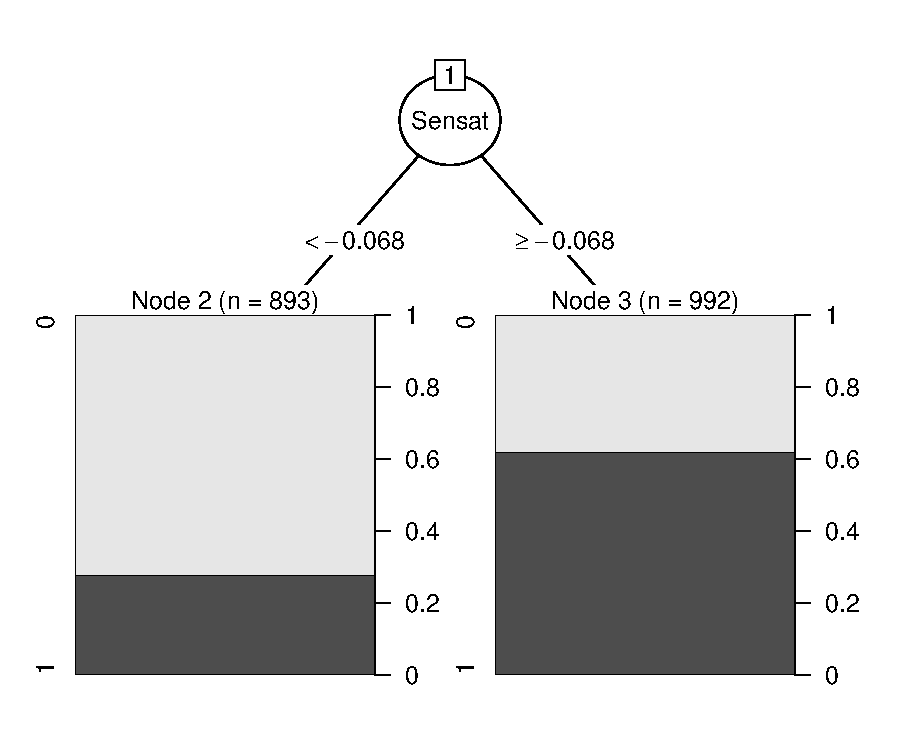
\includegraphics[scale=0.5]{articleV3-decisiontree}
\caption{Decision tree estimated from the full drug data set with ecstasy as response variable.}
\label{fig:Ex1Ttreefulldata}
\end{figure}
The obtained result (as displayed in Figure \ref{fig:Ex1Ttreefulldata}) shows that people with a higher score on Sensation seeking are more at risk for using ecstasy, which makes sense from an intuitive point of view.

To investigate the stability of this result, we create a forest, by drawing 100 bootstrap samples from the original data set and growing a tree on each bootstrap sample:

\begin{example}
R> DrawBoots <- function(dataset, i){
+    set.seed(1234 + i)
+    Boot <- dataset[sample(1:nrow(dataset), size = nrow(dataset), 
+      replace = TRUE), ]
+    return(Boot)
+  }
R> GrowTree <- function(x,y,BootsSample){
+   controlrpart <- rpart.control(minsplit = 100, minbucket = 50,
+    maxdepth = 3, maxsurrogate=0, maxcompete=0)
+   tree <- rpart(as.formula(paste(noquote(paste(y, "~")), noquote(paste(x,
+      collapse = "+")))), data = BootsSample, control = controlrpart)
+   
+   cp <- tree$cptable[order(tree$cptable[1:which.min(tree$cptable[,    
+   "xerror"]), "xerror"]), ]
+   maxcp <- cp[1, "xerror"] + 1.96 * cp[1, "xstd"]
+   cp <- cp[as.numeric(which.max(1 / (maxcp - cp[, "xerror"]))), "CP"]
+  
+   PrunedTree <- prune.rpart(tree, cp = cp) 
+   return(PrunedTree)
+  }
R> set.seed(12345)
R> Boots <- lapply(1:100, function(k) DrawBoots(EcstData, k))
R> Trees <- lapply(1:100, function (i) GrowTree(x = c("Age", "Gender", "Edu",
+   "Neuro", "Extr", "Open", "Agree", "Consc", "Impul", "Sensat"),
+    y = "Ecst", Boots[[i]]))
\end{example} 

To cluster the trees of this forest, we use the \texttt{clusterforest()} function. This requires as input the full originally observed data set and the trees in the forest along with the data sets on which these were based. Furthermore, we should also provide a similarity matrix \textit{or} a similarity measure that is to be used to calculate similarities. In this example, we will let the R-package calculate the similarities using one of the hybrid measures based on predictor-range part occurrences in the definition of leaves with the same class label (see similarity measure No 6 in Table 1). This will allow us to interpret the clustering result in terms of the predictor-related contents of the medoids (viz., in terms of the predictors involved in the definition of each leaf along with a specification of the relevant part of each predictor's range high vs. low) as well as in terms of their class assignments. Finally, we should indicate which cluster solutions we want to explore: We will look at the cluster solutions with one through eight clusters.
\begin{example}

R> set.seed(1)
R> ClusterForest<- clusterforest(observeddata=EcstData,treedata=Boots,
+   trees=Trees, m=6, fromclus=1, toclus=8)
\end{example}

The \texttt{clusterforest()} function returns a \texttt{clusterforest} object. We can use several functions to post-process this result and gain the desired insights. First, we will plot the object to estimate how many clusters are needed to summarize the forest.
\begin{example}
R> plot(ClusterForest)
\end{example}
\begin{figure}[H]
	\centering
	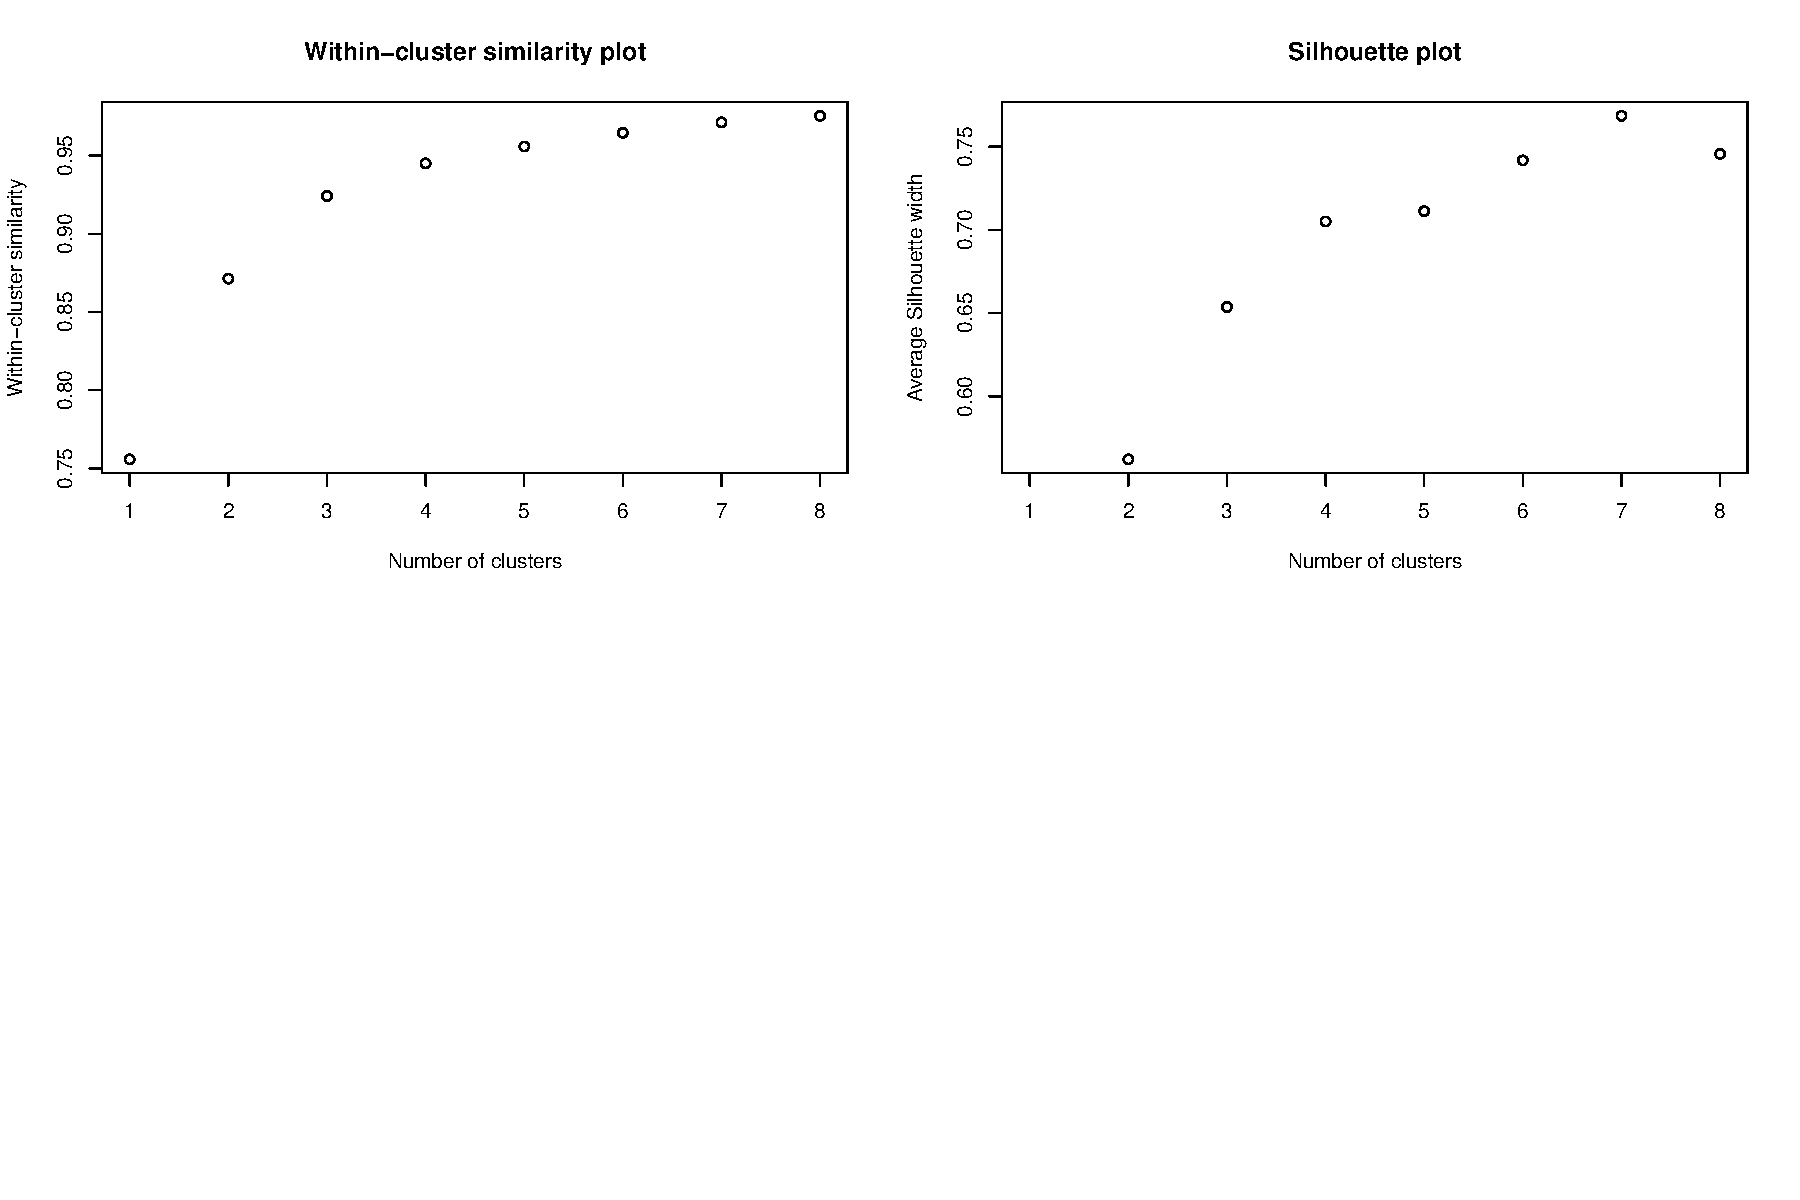
\includegraphics[width=\linewidth, trim= 0 300 20 0, clip]{articleV3-clusters}
	\caption{Average within-cluster similarity and ASW for solutions with 1 through 8 clusters for Example 1 on ecstasy use.}
\label{fig:Ex1Measures}	
\end{figure}

Figure \ref{fig:Ex1Measures} shows for each solution the average within-cluster similarity, and the ASW. The first plot shows that a solution with a relatively small number of clusters (one, two or three) could be sufficient to summarize the forest. The ASW increases until seven clusters, yet the increase flattens out after four clusters. Consequently, in the remainder of this analysis, we will focus on the solutions with one through four clusters.

To understand the central tendency of the forest, we will inspect the cluster medoid of the one-cluster solution. Using the function \texttt{plot()} on a \texttt{clusterforest} object with as second argument a solution number will plot the medoid(s) of the solution in question:
\begin{example}
R> plot(ClusterForest, solution = 1)
\end{example}
The most central tree in the forest is the same as the decision tree that we obtained from the original data set (see Figure \ref{fig:Ex1Ttreefulldata}). 

To evaluate the heterogeneity within the forest, we will first check the cluster medoids and then the cluster sizes for the selected solutions with two, three and four clusters. 
\begin{example}
R> plot(ClusterForest, solution = 2)
R> plot(ClusterForest, solution = 3)
R> plot(ClusterForest, solution = 4)
\end{example}

The cluster medoids for the 1-, 2-, 3-, and 4-cluster solutions are shown in Figures \ref{fig:Ex1Ttreefulldata} and \ref{fig:Ex1Medoids}. (Note that the sample sizes and proportions shown in the leafs of each medoid in Figure \ref{fig:Ex1Medoids} pertain to the bootstrap sample on which the medoid was based and not to the original full data set.) The medoid sets of the different solutions are closely related as: 
\begin{enumerate}
\item All medoids include a root node split on Sensation seeking.
\item All medoids with additional splits under the root node imply one or two further splits of the group scoring high on Sensation seeking.
\item The medoid sets of the 1-, 3-, and 4-cluster solutions are fully nested.
\item Medoid (a) shows up in the 2-, 3-, and 4-cluster solutions. 
\item The second medoid of the 2-cluster solution (i.e., medoid (b), with additional splits on Conscientiousness and Openness) is a kind of a mixture of medoid (c) (in the 3- and 4-cluster solutions, with an additional split on Conscientiousness) and medoid (d) (in the 4-cluster solution, with an additional split on Openness).
\end{enumerate}

\begin{figure}[H]
	\centering
	\begin{subfigure}[t]{.49\textwidth}
		\centering
		\captionsetup{justification=centering}
		\includesvg[width=\linewidth]{fig5a.svg}
		\caption{}	
	\end{subfigure}%
	\begin{subfigure}[t]{.49\textwidth}
		\centering
		\captionsetup{justification=centering}
	\includesvg[width=\linewidth]{Fig5b.svg}
		\caption{}
	\end{subfigure}
	\newline
	
	\begin{subfigure}[t]{.49\textwidth}
		\centering
		\captionsetup{justification=centering}
		\includesvg[width=\linewidth]{fig5c.svg}
		\caption{}
	\end{subfigure}
\begin{subfigure}[t]{.49\textwidth}
	\centering
	\captionsetup{justification=centering}
	\includesvg[width=\linewidth]{fig5d.svg}
	\caption{}
\end{subfigure}

	\caption{Elements of medoid sets of 1-, 2-, 3-, and 4-cluster solution (in addition to Figure \ref{fig:Ex1Ttreefulldata}) for Example 1 on ecstasy use. The ordered medoid sets for the different cluster solutions are as follows. For the 1-cluster solution: $\bigl($Fig. \ref{fig:Ex1Ttreefulldata}$\bigl)$; for the 2-cluster solution: $\bigl($Fig. \ref{fig:Ex1Medoids} (a), Fig. \ref{fig:Ex1Medoids} (b)$\bigl)$; for the 3-cluster solution: $\bigl($Fig. \ref{fig:Ex1Medoids} (a), Fig. \ref{fig:Ex1Ttreefulldata}, Fig. \ref{fig:Ex1Medoids} (c)$\bigl)$; for the 4-cluster solution: $\bigl($Fig. \ref{fig:Ex1Medoids} (a), Fig. \ref{fig:Ex1Ttreefulldata}, Fig. \ref{fig:Ex1Medoids} (c), Fig. \ref{fig:Ex1Medoids} (d)$\bigl)$.}
	\label{fig:Ex1Medoids}
\end{figure}



To determine the sizes of clusters in each solution, we can utilize the \texttt{cluster()} function on the \texttt{clusterforest} object, 
with as second argument the solution number of interest. We combine this with the \texttt{table()} function to count the number of trees assigned to each cluster.
\begin{example}
R> table(clusters(ClusterForest, solution=2))

 1  2 
48 52 

R> table(clusters(ClusterForest, solution=3))

 1  2  3 
44 25 31 

R> table(clusters(ClusterForest, solution=4))

 1  2  3  4 
44 20 27  9 

\end{example}

These figures show that in the 2-, 3-, and  4-cluster solutions almost half of the trees belong to the cluster with Age as secondary splitting variable. Moreover, in the three- and four-cluster solutions, the cluster with Conscientiousness as secondary splitting variable is nonnegligible, too.

Taking all these findings together, the role of Sensation seeking as primary predictor of ecstasy use is without a shadow of doubt. Sensation seeking is the first and only splitting variable in the classification tree estimated from the full data set as well in the medoid of the one-cluster solution. Moreover, it also acts as the primary splitting variable in the subsequent medoids of solutions with two or more clusters. On top of that, we may notice a relatively high proportion of people at risk for ecstasy use in all subgroups of the people scoring high on Sensation seeking. There are indications that, within the group of high sensation seekers, especially younger people (and, to a somewhat lesser extent, people scoring lower on Conscientiousness) are even more at risk for ecstasy use. One might wish to corroborate the latter results on the role of these secondary predictors in follow-up research.


\subsection{Example 2: Predicting Ecstasy use}\label{sec:illustration2}
Whereas the goal of the first analysis was to find out which types of persons are at risk of using ecstasy, the goal of the second analysis is to \textit{predict} (as accurately as possible) whether a person is at risk of using ecstasy. As the accuracy of ensemble methods is normally higher than that of single decision trees, we will revert to a random forest to address this objective. In line with the "Explainable AI" movement \citep{Arrieta2020}, we will subsequently use C443 to get insight into this random forest. 

We use the same data as in the previous section, split it into a training and test set, and then fit a random forest on the training set using the \pkg{randomForest} package. Note that we could also have used the \pkg{ranger} package for this application. We limit the maximum number of nodes of each tree to six (to facilitate the interpretation of individual trees) and use default settings for the hyperparameters.

\begin{example}
R> EcstData$Ecst <- as.factor(EcstData$Ecst)
R> train.id <- sample(nrow(EcstData), 3/4 * nrow(EcstData))
R> EcstData.train <- EcstData[train.id, ]
R> EcstData.test <- EcstData[-train.id, ]

R> DrugsRF <- randomForest(Ecst ~ ., data = EcstData.train, importance = TRUE,
+   proximity = TRUE, keep.inbag = T, maxnodes = 6,ntree = 500)


R> preds_test=predict(DrugsRF,EcstData.test)
R> preds_train=predict(DrugsRF,EcstData.train)

R> mean(preds_test==EcstData.test$Ecst)
[1] 0.6779661
R> mean(preds_train==EcstData.train$Ecst)
[1] 0.7296532
\end{example}
The prediction acccuracy of the random forest on the training set is 0.73, and on the test set 0.68.

Next, we cluster the trees in the forest using C443 with the same similarity measure as in the previous section (as it takes into account both the trees' meaning and classifications). We evaluate solutions with up to 20 clusters. 
\begin{example}
R> set.seed(1)
R> ClusterForest<- clusterforest(observeddata = EcstData.train, trees = DrugsRF, 
+                              m = 6, fromclus = 1, toclus = 20)
R> plot(ClusterForest, predictive_plots=TRUE )
\end{example}
The plot function with \texttt{predictive\_plots=TRUE} allows us to compare the different solutions in terms of their accuracy on the training set, as well as in terms of the agreement in the predictions with the random forest as a whole. The plot with Accuracy shows us that even with the one cluster solution, the accuracy on the training set is close to that of the random forest. The agreement in predictions is above 90\% starting from the two-cluster solution. 


\begin{figure}[H]
	\centering
	\begin{subfigure}[t]{.49\textwidth}
		\centering
		\captionsetup{justification=centering}
		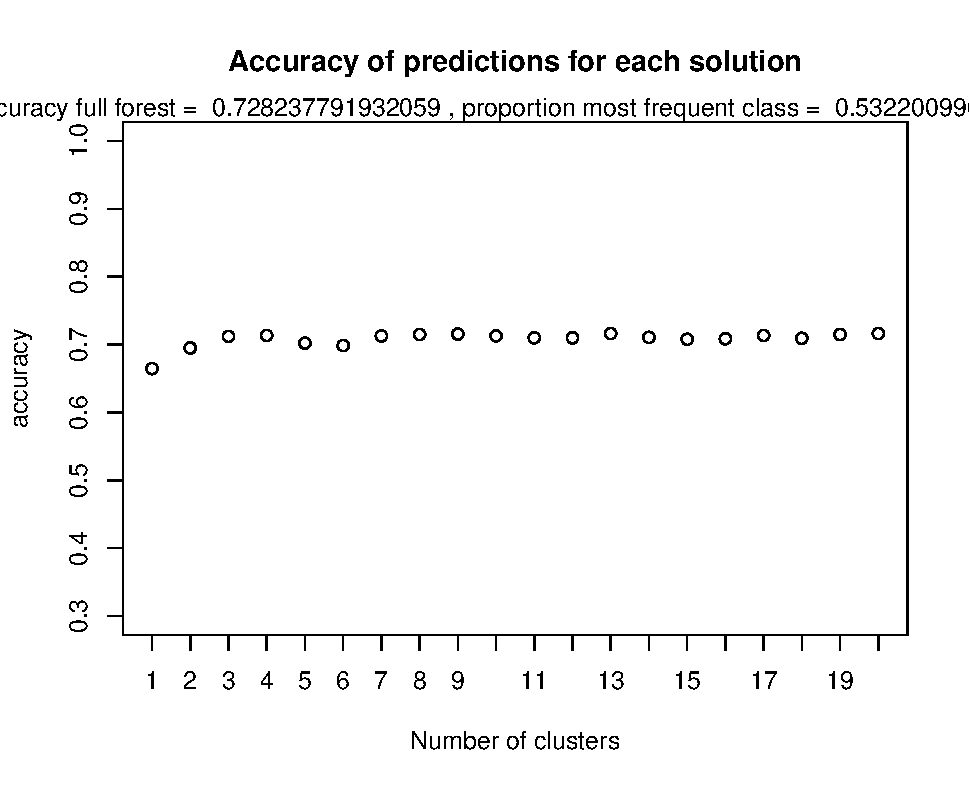
\includegraphics[width=\linewidth, trim=0 0 0 2.02cm, clip]{accuracy}
		\caption{}	
	\end{subfigure}%
	\begin{subfigure}[t]{.49\textwidth}
		\centering
		\captionsetup{justification=centering}
	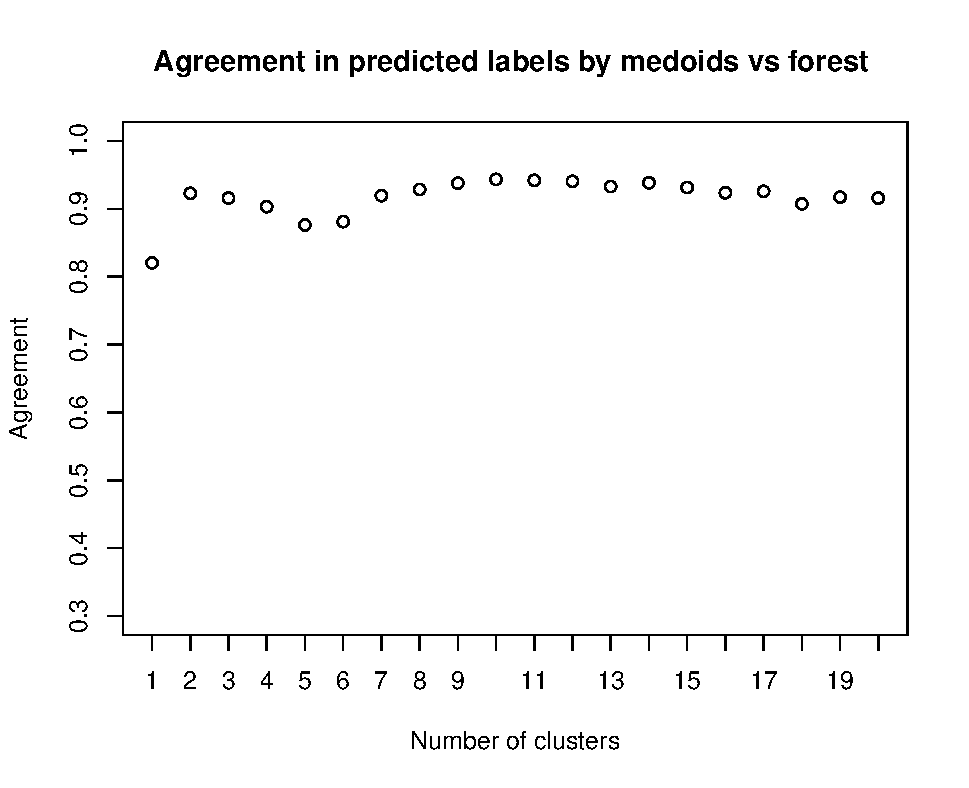
\includegraphics[width=\linewidth, trim=0 0 0 2.02cm, clip]{agreement}
		\caption{}
	\end{subfigure}
		\caption{Plots to evaluate the different clustering solutions, with (a) the accuracy on the training dataset for each clustering solution and (b) the agreement of predictions between a given cluster solution and the full forest. }
	\label{fig:Ex2Measures}
\end{figure}



As the accuracy on the training set is improving up and until the three cluster solution, we plot the medoids of this solution.   
\begin{example}
R> plot(ClusterForest, solution = 3)
\end{example}

\begin{figure}[H]
	\centering
	\begin{subfigure}[t]{.49\textwidth}
		\centering
		\captionsetup{justification=centering}
		\includesvg[width=\linewidth]{fig7a.svg}
		\caption{}	
	\end{subfigure}%
	\begin{subfigure}[t]{.49\textwidth}
		\centering
		\captionsetup{justification=centering}
	\includesvg[width=\linewidth]{fig7b.svg}
		\caption{}
	\end{subfigure}
	\newline
	
	\begin{subfigure}[t]{.49\textwidth}
		\centering
		\captionsetup{justification=centering}
		\includesvg[width=\linewidth]{fig7c.svg}
		\caption{}
	\end{subfigure}

	\caption{Medoids of the  3-cluster solution for Example 2 on ecstasy use.}
	\label{fig:Ex2Medoids}
\end{figure}
In the first two medoids, Figure \ref{fig:Ex2Medoids} (a) and (b), for one of the terminal nodes only, the class assignment is 1 (i.e., ecstasy use). In the first medoid this is the case for people with Sensation Seeking >-0.068 and Age $\leq$ 0.796, in the second medoid this is the case for people with Openness >-0.248 and Age $\leq$ 0.796. There is a correlation between Sensation Seeking and Openness, and, indeed, when looking at the class assignments of these two medoids, it turns out that they are for a large part overlapping:
\begin{example}
R> table(EcstData.train$Age<=0.796 & EcstData.train$Sensat>-0.068,
EcstData.train$Age<=0.796 & EcstData.train$Open>-0.248)
        FALSE TRUE
  FALSE   556  201
  TRUE    162  494
\end{example}
In the third medoid, two terminal nodes are assigned to class 1, namely:  1) the node where Openness >0.217 and Sensation Seeking >-0.371, and 2) the node where Openness $\leq$ 0.217 and  Sensation seeking >-0.68 and Conscientiousness $\leq$ 0.191.

Finally, we estimate the accuracy of the three-cluster solution (where the predicted class is the average of the predicted class by each medoid tree weighted by the number of trees assigned to its cluster) on the test set, and compare it to that of the random forest as a whole. We also check the agreement between the predictions of the two on the test set. To do so, we use the randomForest2party function (an internal function of the R-package) to transform the two medoid trees of the forest into a party object. 
\begin{example}
R> table(clusters(ClusterForest,solution=3))
  1   2   3 
191 133 176 
R> tree310=C443:::randomForest2party(EcstData.train, DrugsRF, ClusterForest$medoids[[3]][1])
R> tree329=C443:::randomForest2party(EcstData.train, DrugsRF, ClusterForest$medoids[[3]][2])
R> tree453=C443:::randomForest2party(EcstData.train, DrugsRF, ClusterForest$medoids[[3]][3])

preds_test310=predict(tree310,EcstData.test )
preds_test329=predict(tree329,EcstData.test )
preds_test453= predict(tree453,EcstData.test )
preds_total = round(((as.numeric(preds_test310)-1)*table(clusters(ClusterForest,solution=3))[1]+
(as.numeric(preds_test329)-1)*table(clusters(ClusterForest,solution=3))[2]+
(as.numeric(preds_test453)-1)*table(clusters(ClusterForest,solution=3))[3])/500 , 0)

R> mean(preds_total==EcstData.test$Ecst)
[1]  0.6716102
R> mean(preds_total==preds_test)
[1] 0.9088983

\end{example}
As a relatively similar number of trees is assigned to each cluster, the prediction of the three cluster solution comes down to a majority vote. It turns out that also on the test data set, the accuracy is very similar to that of the full forest (67\% compared to 68\% for the full forest), and the agreement of predictions with the full forest is still around 91\%. Therefore, in the current example,  without losing much predictive power, one could use a summarized forest with only three trees instead of a forest with 500 trees. 



\subsection{Example 3: Multiple outcome variables} \label{sec:illustration3}
The goal of our analysis in this third example is to find out which are the common and distinctive psychological mechanisms for being at risk for using different drugs (amphetamines, benzodiazepines, ecstasy, LSD and mushrooms). To answer this question, we will draw 100 bootstrap samples for each drug, and grow a classification tree on each sample. Subsequently, we will use \pkg{C443} to calculate similarities between these trees, and cluster them. Finally, we will post-process the obtained clustering result to answer the question outlined above. 
 
We start by creating a separate data set for each drug:
\begin{example}
R> AmphetData <- drugs[, c("Age", "Gender", "Edu", "Neuro", "Extr", "Open", 
+    "Agree", "Consc", "Impul", "Sensat", "Amphet")]
> BenzoData <- drugs[, c("Age", "Gender", "Edu", "Neuro", "Extr", "Open", 
+    "Agree","Consc", "Impul", "Sensat", "Benzos")]
> EcstData <- drugs[, c("Age", "Gender", "Edu", "Neuro", "Extr", "Open", 
+    "Agree", "Consc", "Impul", "Sensat", "Ecst")]
> LSDData <- drugs[, c("Age", "Gender", "Edu", "Neuro", "Extr", "Open", 
+    "Agree", "Consc", "Impul", "Sensat", "LSD")]
> MushData <- drugs[, c("Age", "Gender", "Edu", "Neuro", "Extr", "Open", 
+    "Agree", "Consc", "Impul", "Sensat", "Mush")]
\end{example}

Next, for each drug, we draw the bootstrap samples and grow a tree on every sample. We use the \texttt{DrawBoots} and \texttt{GrowTree} functions (already used in Example 1) to do so:
\begin{example}

R> BootsAmphet <- lapply(1:100, function(k) DrawBoots(AmphetData, k))
R> set.seed(123456)
R> TreesAmphet <- lapply(1:100, function (i) GrowTree(x = c("Age", "Gender", "Edu",   
+    "Neuro", "Extr", "Open", "Agree", "Consc", "Impul", "Sensat"), y="Amphet", BootsAmphet[[i]]))

> BootsBenzo <- lapply(1:100, function(k) DrawBoots(BenzoData, k))
> set.seed(123456)
> TreesBenzo <- lapply(1:100, function (i) GrowTree(x = c("Age", "Gender", "Edu", "Neuro", "Extr",
+    "Open", "Agree", "Consc", "Impul", "Sensat"), y = "Benzos", BootsBenzo[[i]]))
> 
> BootsEcst <- lapply(1:100, function(k) DrawBoots(EcstData, k))
> set.seed(123456)
> TreesEcst <- lapply(1:100, function (i) GrowTree(x = c("Age", "Gender", "Edu", "Neuro", "Extr",  
+    "Open", "Agree", "Consc", "Impul", "Sensat"), y="Ecst",  BootsEcst[[i]]))
> 
> BootsLSD <- lapply(1:100, function(k) DrawBoots(LSDData, k))
> set.seed(123456)
> TreesLSD <- lapply(1:100, function (i) GrowTree(x = c("Age", "Gender", "Edu", "Neuro", "Extr", 
+    "Open", "Agree", "Consc", "Impul", "Sensat"), y = "LSD", BootsLSD[[i]]))
> 
> BootsMush <- lapply(1:100, function(k) DrawBoots(MushData, k))
> set.seed(123456)
> TreesMush <- lapply(1:100, function (i) GrowTree(x = c("Age", "Gender", "Edu",  "Neuro", "Extr", 
+    "Open", "Agree", "Consc", "Impul", "Sensat"), y = "Mush",  BootsMush[[i]]))

\end{example}


We then create one list with all data sets, and one list with all trees.
\begin{example}
R> Boots <- c(BootsAmphet, BootsBenzo, BootsEcst, BootsLSD, BootsMush)
R> Trees <- c(TreesAmphet, TreesBenzo, TreesEcst, TreesLSD, TreesMush)
\end{example}

We use the resulting forest as input for the \texttt{clusterforest()} function. We also provide a vector with a covariate value of each tree, that is to say, the response variable (drug) on which the tree was based. We choose the same similarity measure as in Example 1.
\begin{example}
R> set.seed(1)
R> ClusterForestMultiple <- clusterforest(observeddata=drugs,treedata=Boots, trees=Trees, 
+    m=6, fromclus=1, toclus=8, treecov=rep(c("Amphet", "Benzo", "Ecst",
+    "LSD", "Mush"), each = 100)) 
\end{example}

Again, we use the \texttt{plot()} function to estimate the number of clusters needed to summarize the forest:
\begin{example}
R> par(mfrow = c(2, 2))
R> plot(ClusterForestMultiple) 
\end{example}

\begin{figure}[H]
	\centering
	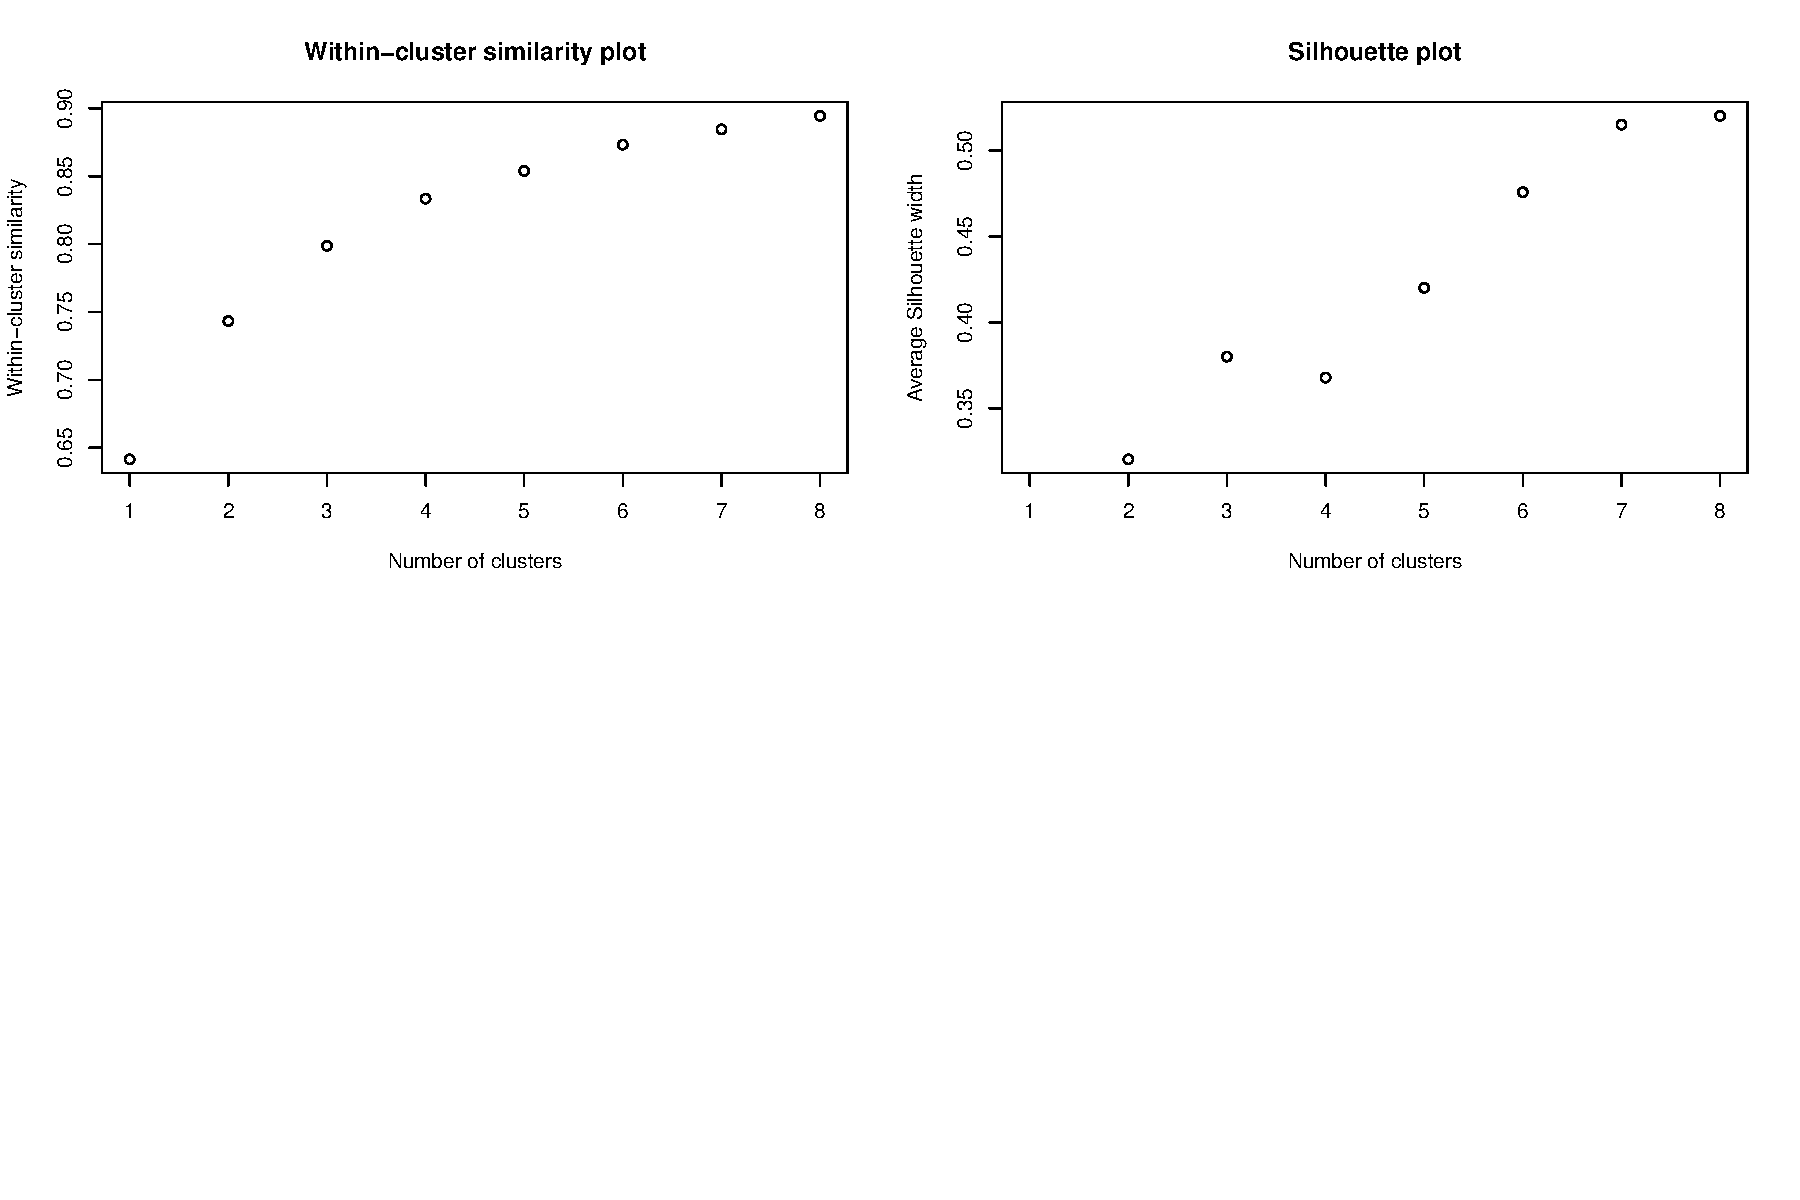
\includegraphics[width=\linewidth, trim= 0 300 20 0, clip]{articleV3-plotnrclust}
	\caption{Average within-cluster similarity and ASW for solutions with 1 through 8 clusters for Example 3 on use of amphetamines, benzodiazepines, ecstasy, LSD and mushrooms.}
	\label{fig:Ex3Measures}	
\end{figure}

The two plots (Figure \ref{fig:Ex3Measures}) to do not clearly point at an optimal solution. Although the ASW plot seems to favor solutions with a higher number of clusters, the three-cluster solution may be interesting to explore, because its ASW stands out compared to the 2- and 4-cluster solutions. All things considered, this seems to be an interesting parsimonious solution for further examination. We will do so from the point of view of the relation between the clustering and the type of drug at the basis of each tree in the forest, both in extensional terms (viz., with regard to the relation between cluster membership and the type of response variable underlying each of the trees in the forest) and in intensional terms (viz., with regard to the relation between medoid contents and the substantive nature of each of the response variables).

To understand the relation between the clusters' extension and the type of response variable underlying each of the trees in the forest, we will count for each response variable the number of trees that have been assigned to each cluster. This will provide insight into whether the trees of the same versus different response variables mostly end up in the same versus in different clusters. As such, this may clarify whether there is a relationship between the nature of the drug and the clustering's extension, while factoring in tree instability (as reflected by whether trees based on the same drug consistently belong to the same cluster or not). We do this using the \texttt{treesource} function:
\begin{example}
R> treesource(ClusterForestMultiple, solution= 3)
\end{example}

\begin{figure}[H]
	\centering
    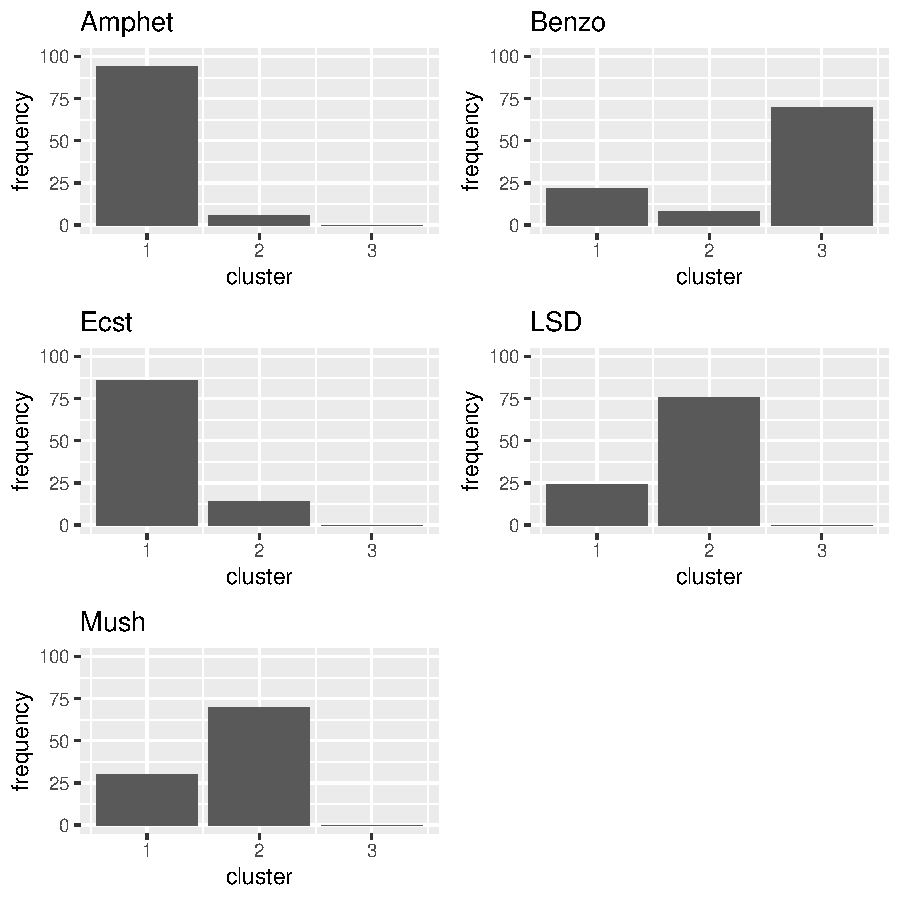
\includegraphics[scale=0.7]{articleV3-treesource3}
	\caption{For each response variable frequencies of associated trees that were assigned to each of the clusters of the three-cluster solution for Example 3 on use of amphetamines, benzodiazepines, ecstasy, LSD and mushrooms.}
	\label{fig:Ex3Frequencies}	
\end{figure}

From the result, we may conclude that the trees of most response variables are relatively stable (in the sense that for most response variables a clear majority of the trees is assigned to one specific cluster). Furthermore, it is interesting to note that the trees of the two stimulant drugs (viz., ecstasy and amphetamines) mainly end up in the same cluster and that the same holds for the trees of the two hallucinant drugs (viz., mushrooms and LSD). Conversely, the trees of the single tranquilizing drug (viz., benzodiazepines) mostly end up in a separate cluster.

To clarify the intensional relation between the clustering and the substantive nature of each of the response variables, we first plot the medoids of the three-cluster solution.
\begin{example}
R> plot(ClusterForestMultiple, solution = 3)
\end{example}


The first, second and third medoid are shown in Figure \ref{fig:Ex3Medoids}. The medoids, along with the cluster membership frequencies of Figure \ref{fig:Ex3Frequencies}, imply that Sensation seeking plays an important role in being at risk for using the two stimulant drugs (i.e., ecstasy and amphetamines, see Figure \ref{fig:Ex3Medoids} (a)). To be at risk for using the hallucinatory drugs (LSD and mushrooms), apart from a higher score on Sensation seeking, also a higher score on Openness to experience is needed (Figure \ref{fig:Ex3Medoids} (b)). Finally, for using benzodiazepines (the only tranquilizing group of drugs), Neuroticism seems to play a key role, with people scoring higher on the Neuroticism scale being more at risk for using the drugs in question (Figure \ref{fig:Ex3Medoids} (c)). All in all, from this analysis, we may derive that there is some overlap in the types of people that are at risk for using the different drugs under study, with personality characteristics differentiating in a meaningful way between people susceptible to the use of stimulant, hallucinatory, and tranquilizing substances.
\begin{figure}[H]
	\centering
		\begin{subfigure}[t]{.49\textwidth}
		\centering
		\captionsetup{justification=centering}
		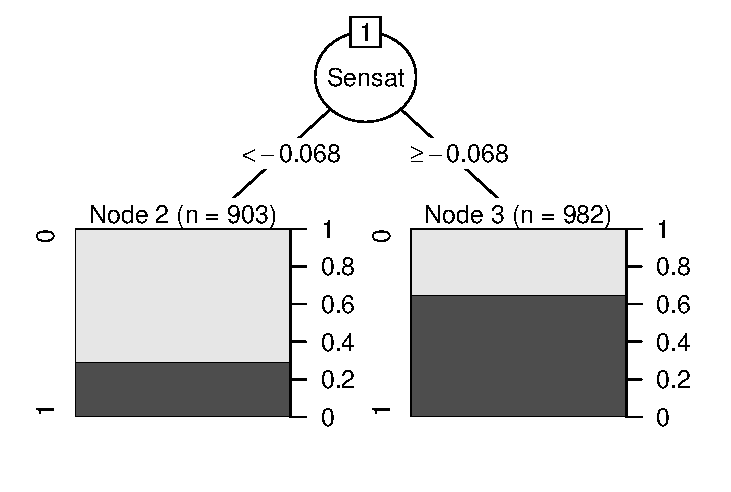
\includegraphics[width=\linewidth, trim=0 20 0 0, clip]{MO_M1.pdf}
		\caption{}
	\end{subfigure}
	\begin{subfigure}[t]{.49\textwidth}
		\centering
		\captionsetup{justification=centering}
		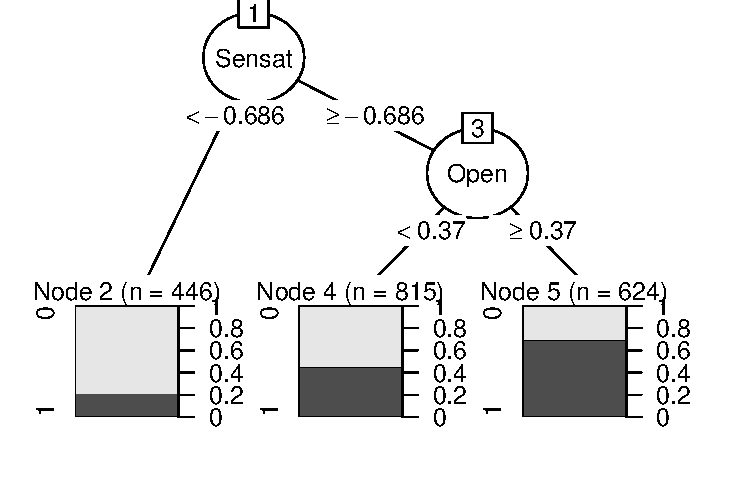
\includegraphics[width=\linewidth, trim=0 20 0 0, clip]{MO_M2.pdf}
		\caption{}
	\end{subfigure}
\newline
\begin{subfigure}[t]{.49\textwidth}
	\centering
	\captionsetup{justification=centering}
	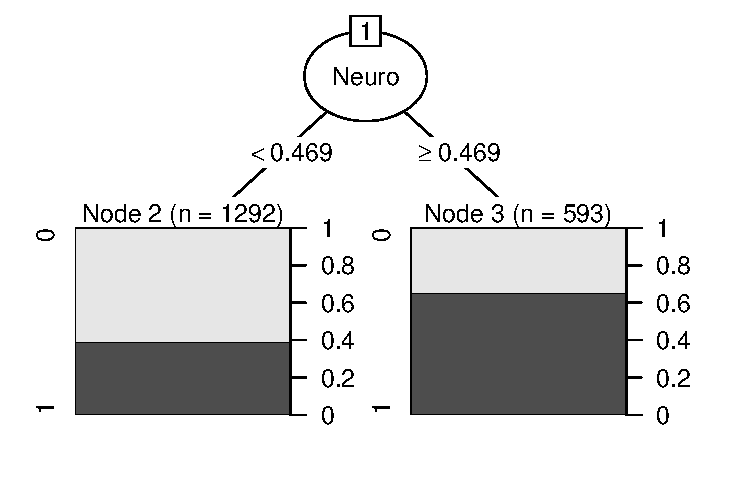
\includegraphics[width=\linewidth, trim=0 20 0 0, clip]{MO_M3.pdf}
	\caption{}
\end{subfigure}
	\caption{The first, second and third medoid of the three-cluster solution for Example 3 on use of amphetamines, benzodiazepines, ecstasy, LSD and mushrooms.}
	\label{fig:Ex3Medoids}
\end{figure}

%% -- Summary/conclusions/discussion -------------------------------------------

\section{Concluding remark} \label{sec:summary}
In this paper we presented the R-package \pkg{C443}, which solves a major problem of trees (viz., their lack of stability) and a major problem of forests (viz., their black box nature). \pkg{C443} is well accessible by accepting as input trees produced by a broad range of R-packages, including all possible trees that are stored as party objects or that are convertible into such objects, including ranger and randomForest objects. Moreover, the package is also versatile by both allowing to make an appeal to in-built tools for calculating various tree similarity measures and by accepting as input all possible user-provided tree similarities. In the same vein, the package includes a comprehensive set of in-built tools to postprocess the 
results generated by the methodology, and allows for the integration of other user-provided postprocessing tools. \pkg{C443} operates via an optimal involvement of and synergy with neighboring R-packages such as \pkg{partykit},  \pkg{randomForest}, \pkg{ranger}  and \pkg{cluster}. As a bonus, the internal functions C443:::randomForest2party and C443:::ranger2party can also be applied outside the context of C443 to print, plot, or post-process trees obtained from the  \pkg{randomForest} or \pkg{ranger} packages.
As further illustrated by three applications, \pkg{C443} is user-friendly and may yield various insights into forests of classification trees and classification-related questions.% Otherwise, whereas the two above applications pertained to the evaluation of tree stability in case of one or multiple outcomes, the C443 package may be useful in quite different contexts as well. For instance, on may think of a forest that was created to increase prediction accuracy (e.g., a random forest). In such a case, C443 could help to gain insight into the random forest, with the additional option to strike a compromise between insightfulness and prediction accuracy. In particular, the latter could be achieved by choosing the number of clusters on the basis of a plot of the agreement between the predicted class labels for all objects based on the random forest as a whole, versus based on the first k medoid trees only (weighted by their cluster cardinalities).



\section*{Acknowledgments}
The research reported in this paper was supported in part by the Research Foundation - Flanders (G080219N and K802822N) and by the Research Fund of KU Leuven (C14/19/054). The data used in the illustrative applications were obtained from the UCI Machine Learning Repository \citep{Dheeru2017,Fehrman2017}.

\bibliography{RJreferences}

\address{Aniek Sies\\
  KU Leuven, Faculty of Psychology and Educational Sciences\\
  Tiensestraat 102 - Box 3713\\
  3000\\
  Belgium\\
  \email{aniek.sies@kuleuven.be}}

\address{Iven Van Mechelen\\
  KU Leuven, Faculty of Psychology and Educational Sciences\\
\email{iven.vanmechelen@kuleuven.be}}
